% \qiying{Comment like this}

% \hao{Comment like this}

% \zheng{Comment like this}

% \weinan{Comment like this}

% \hongli{Comment like this}
\vspace{-20pt}
\begin{figure}[h]
    \centering
    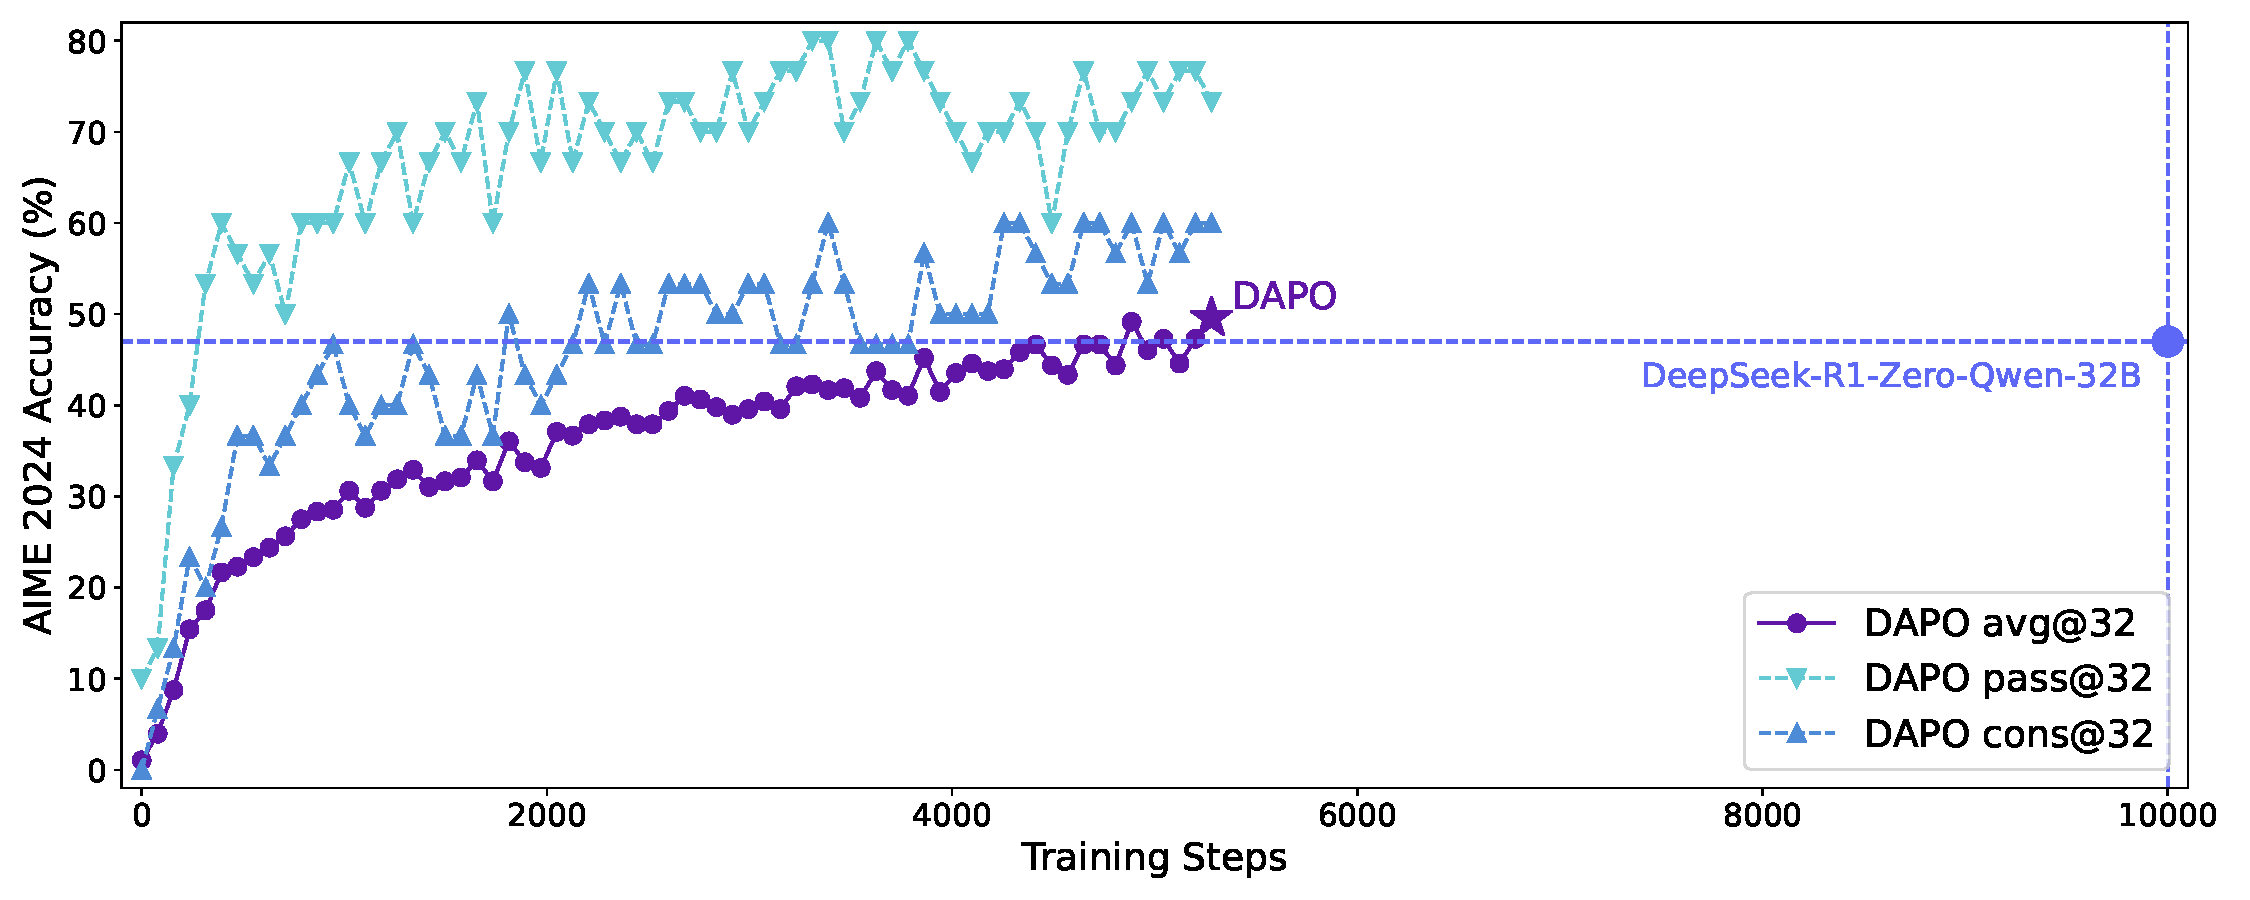
\includegraphics[width=0.92\linewidth]{figures/score.pdf}
    \caption{AIME 2024 scores of \method on the Qwen2.5-32B base model, outperforming the previous SoTA DeepSeek-R1-Zero-Qwen-32B using 50\% training steps.}
    \label{fig:front}
\end{figure}

\newpage
\section{Introduction}

Test-time scaling such as OpenAI's o1~\cite{o1} and DeepSeek's R1~\cite{guo2025deepseek} brings a profound paradigm shift to Large Language Models (LLMs)~\cite{gpt4,claude35sonnet,gpt3,chowdhery2023palm,dsv3}. Test-time scaling enables longer Chain-of-Thought thinking and induces sophisticated reasoning behaviors, which makes the models superior in competitive math and coding tasks like AIME and Codeforces.

The central technique driving the revolution is large-scale Reinforcement Learning (RL), which elicits complex reasoning behaviors such as self-verification and iterative refinement. However, the actual algorithm and key recipe for scalable RL training remains a myth, hidden from technical reports of existing reasoning models~\cite{o1,guo2025deepseek,grok,gemini-thinking,qwq,k1.5}. In this paper, we reveal significant obstacles in large-scale RL training and open-source a scalable RL system with fully open-sourced algorithm, training code and dataset that provides democratized solutions with industry-level RL results. 

We experiment over Qwen2.5-32B~\cite{yang2024qwen2} as the pretrained model for RL. In our initial GRPO run, we achieved only 30 points on AIME — a performance significantly below DeepSeek’s RL (47 points). A thorough analysis reveals that the naive GRPO baseline suffers from several key issues such as entropy collapse, reward noise, and training instability. The broader community has encountered similar challenges in reproducing DeepSeek's results~\cite{rendarl,OpenReasonerZero2025,hu2025reinforce++,cui2025process,lee2024token,kazemnejad2024vineppo,yuan2025s} suggesting that critical training details may have been omitted in the R1 paper that are required to develop an industry-level, large-scale, and reproducible RL system.

To close this gap, we release an open-source state-of-the-art system for large-scale LLM RL, which achieves 50 points on AIME 2024 based on Qwen2.5-32B model, outperforming previous state-of-the-art results achieved by DeepSeek-R1-Zero-Qwen-32B~\cite{guo2025deepseek} (47 points) using 50\% training steps (Figure~\ref{fig:front}). We propose the \textbf{D}ecoupled Clip and \textbf{D}ynamic s\textbf{A}mpling \textbf{P}olicy \textbf{O}ptimization (\textbf{DAPO}) algorithm, and introduce 4 key techniques to make RL shine in the long-CoT RL scenario. Details are presented in Section~\ref{sec:method}.
\begin{enumerate}
    \item \textbf{Clip-Higher}, which promotes the diversity of the system and avoids entropy collapse;
    \item \textbf{Dynamic Sampling}, which improves training efficiency and stability;
    \item \textbf{Token-Level Policy Gradient Loss}, which is critical in long-CoT RL scenarios;
    \item \textbf{Overlong Reward Shaping}, which reduces reward noise and stabilizes training.
\end{enumerate}
Our implementation is based on verl~\cite{sheng2024hybridflow}. By fully releasing our state-of-the-art RL system including training code and data, we aim to reveal valuable insights to large-scale LLM RL that benefit the larger community.
